\section{Implementierung}
In diesem Abschnitt befassen wir uns mit den wesentliche Implementierungs\-/Details
der zu dieser Arbeit begleitenden Software.

\subsection{Überblick}

\subsection{Atomorbitale und Basis\-/funktionen}\label{basis-functions-section}
Wir befassen uns nun genauer mit den verwendeten Atomorbitalen.
Wie am Anfang des letzten Kapitels beschrieben, werden Atomorbitale verwendet,
um die Molekülorbitale darzustellen. In diesem Kontext werden die Atomorbitale
Basisfunktionen genannt und die Menge der verwendeten Basisfunktionen
ist der so genannte Basis\-/Satz.

Es werden üblicherweise zwei Arten von Basisfunktionen verwendet,
um Atomorbitale zu konstruieren:

\begin{enumerate}
    \item Slater-Type-Orbitals (STO)\\
    STOs werden durch die analytischen Lösungen des Wasserstoff\-/Atoms dargestellt
    und können deshalb die Wellenfunktionen von Atomen sehr genau repräsentieren.
    Jedoch fällt die Berechnung der 2\-/Elektronen\-/Integrale schwer,
    weshalb die Verwendung von so genannten GTOs bevorzugt wird.
    \item Gaussian-Type-Orbitals (GTO)\\
    Wie der Name schon bereits sagt, werden Gauss-Funktionen verwendet,
    um die genaueren STOs zu approximieren. Im Gegensatz zu den STOs ist
    die Evaluierung der 2\-/Elektronen\-/Integrale mit GTOs viel leichter.
    GTOs werden durch die folgende kartesische Form definiert:\\
    \begin{equation}
        \chi(x,y,z) = N \cdot x^i y^j z^k \cdot \exp (-\alpha (x^2+y^2+z^2))
    \end{equation}

    Die Parameter $i,j,k$ entscheiden über die Art und Form des Orbitals (S, P, D ...).
    Die restlichen Parameter $N, \alpha$ dienen der Normierung und Anpassung der Größe des Orbitals.

    \begin{figure}[h]
        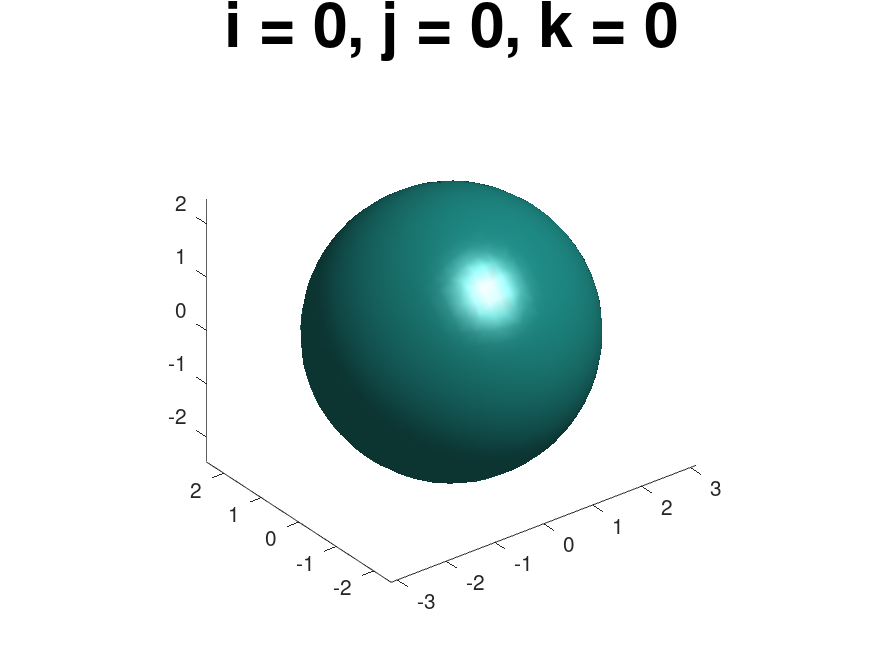
\includegraphics[trim=50 0 50 0, clip, width=0.24\textwidth]{res/GTOs/ao_0_0_0.png}
        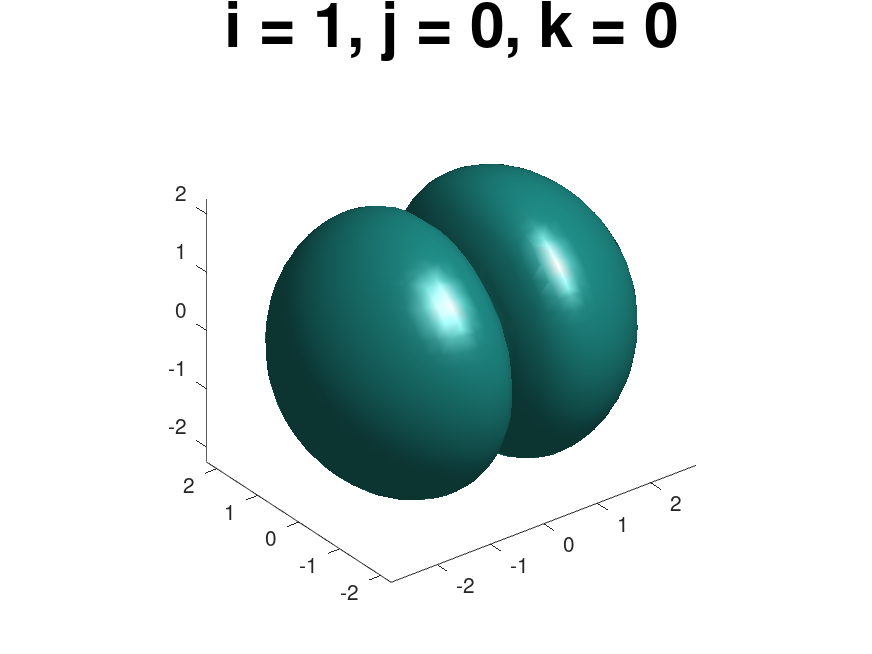
\includegraphics[trim=50 0 50 0, clip, width=0.24\textwidth]{res/GTOs/ao_1_0_0.png}
        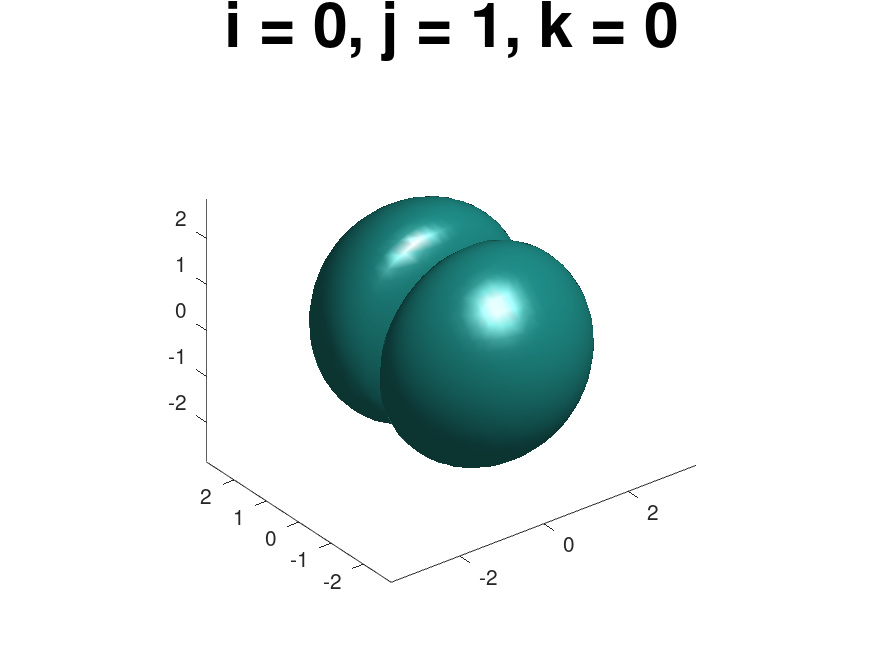
\includegraphics[trim=50 0 50 0, clip, width=0.24\textwidth]{res/GTOs/ao_0_1_0.png}
        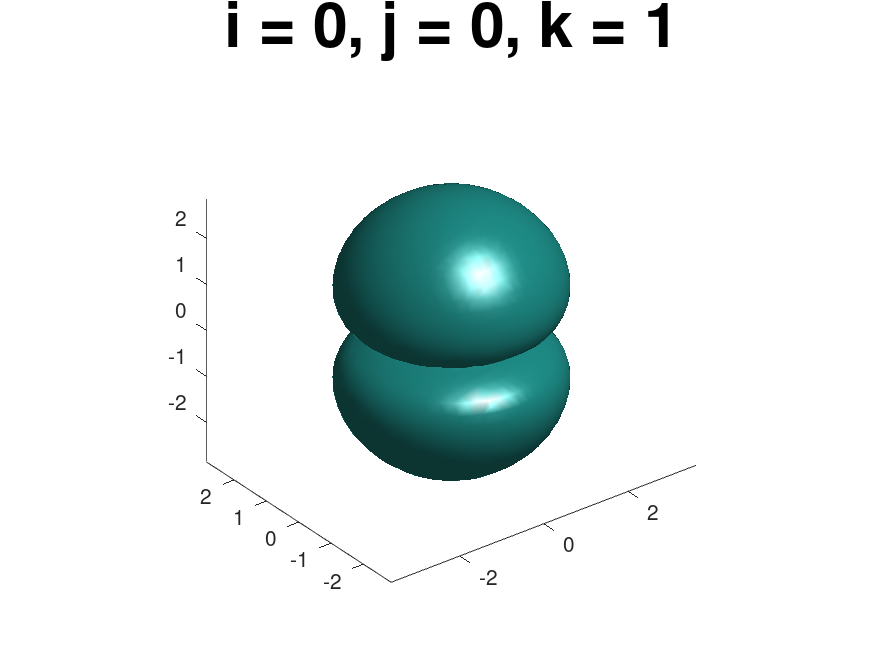
\includegraphics[trim=50 0 50 0, clip, width=0.24\textwidth]{res/GTOs/ao_0_0_1.png}
        \caption{GTOs des S-Orbitals und der drei P-Orbitale mit $N=2$ und $\alpha = 0.5$}
    \end{figure}

    TODO cite essentials of computational chemistry.
\end{enumerate}

In der Implementierung werden GTOs verwendet, aufgrund der leichteren Integral\-/Berechnung,
welche im \cref{repulsion-integrals-section} genauer behandelt wird.
Im Programm werden die Parameter der GTOs aus Dateien mit vorgefertigten Basissätzen extrahiert.
In diesen Dateien gibt es für jedes Atom Parameter zur Konstruktion der relevanten GTOs.
Bei GTOs ist es außerdem üblich, dass eine Linearkombination mehrere GTOs verwendet wird 
zur Beschreibung eines Atomorbitals, diese Kombination von GTOs wird ein Contracted GTO (CGTO) genannt.
CGTOs verhalten sich ähnlich zu GTOs und werden deshalb nicht gesondert behandelt.

\subsection{Schätzung der Start-Orbitale}
Im SCF\-/Verfahren wird eine Start\-/Schätzung benötigt, um überhaupt mit dem iterativen Prozess anzufangen.
Es wurde sich für die leichteste Approximation entschieden, welche die Koeffizienten alle null setzt.
Dies kommt einem Iterationsschritt gleich,
bei dem jegliche Elektron\-/Elektron\-/Interaktionen vernachlässigt werden.
Es werden also effektiv nur die Atomorbitale jedes Atoms konstruiert
und als Ansatz für die Rechnung genommen. Im Rahmen dieser Arbeit genügt diese simple Approximation,
da ebenfalls nur einfache Moleküle betrachtet werden.

\subsection{Berechnung der Repulsions\-/Integrale}\label{repulsion-integrals-section}